% Preambel mit Einstellungen importieren
% Document type and used packages
\documentclass[open=right, % Sorgt für Umbruch bei Chapter (any erzeugt keine Leerseiten) -> Kapitel darf nur auf der rechten Seite beginnen
    paper=A4,               % DIN-A4-Papier
    a4paper,                % DIN-A4-Papier
    12pt,                   % Schriftgöße
    headings=small,         % Kleine Überschriften
    headsepline=true,       % Trennlinie am Kopf der Seite
    footsepline=false,      % Keine Trennlinie am Fuß der Seite
    bibliography=totoc,     % Literaturverzeichnis in das Inhaltsverzeichnis aufnehmen
    twoside=off,            % Für doppelseitigen Druck auf on stellen, off für einseitig
    DIV=7,                  % Verhältnis der Ränder zum bedruckten Bereich
    chapterprefix=false,    % Kapitel x vor dem Kapitelnamen
    numbers=noendperiod,    % kein Punkt am Ende der Nummerierung
    cleardoublepage=plain]{scrbook}

% Pakete einbinden, die benötigt werden
\usepackage{scrlayer-scrpage}
\usepackage[utf8]{inputenc}       % Dateien in UTF-8 benutzen
\usepackage[T1]{fontenc}          % Zeichenkodierung
\usepackage{graphicx}             % Bilder einbinden
\usepackage[main=ngerman, english]{babel}       % Deutsch und Englisch unterstützen
\usepackage{xcolor}               % Color support
\usepackage{amsmath}              % Matheamtische Formeln
\usepackage{amsfonts}             % Mathematische Zeichensätze
\usepackage{amssymb}              % Mathematische Symbole
\usepackage{float}                % Fließende Objekte (Tabellen, Grafiken etc.)
\usepackage{booktabs}             % Korrekter Tabellensatz
\usepackage[printonlyused, withpage, footnote]{acronym}  % Abkürzungsverzeichnis [nur verwendete Abkürzugen]
\usepackage{makeidx}              % Sachregister
\usepackage{listings}             % Source Code listings
\usepackage{listingsutf8}         % Listings in UTF8
\usepackage[hang,font={sf,footnotesize},labelfont={footnotesize,bf}]{caption} % Beschriftungen
\usepackage[scaled]{helvet}       % Schrift Helvetia laden
\usepackage[absolute]{textpos}	  % Absolute Textpositionen (für Deckblatt)
\usepackage{calc}                 % Berechnung von Positionen
\usepackage{blindtext}            % Blindtexte
\usepackage[left=30mm,right=25mm,top=25mm,bottom=25mm]{geometry} % Ränder ändern
\usepackage{setspace}             % Abstände korrigieren
\usepackage{ifthen}               % Logische Bedingungen mit ifthenelse
\usepackage{scrhack}              % Get rid of tocbasic warnings
\usepackage[pagebackref=false,german]{hyperref}  % Hyperlinks
\usepackage[all]{hypcap}          % Korrekte Verlinkung von Floats
\usepackage[autostyle=true,german=quotes]{csquotes}   % Zitate
\usepackage[backend=biber,
  isbn=true,                     % ISBN nicht anzeigen, gleiches geht mit nahezu allen anderen Feldern
  %sortlocale=de_DE,               % Sortierung der Einträge für Deutsch
  sortlocale=en_US,              % Sortierung der Einträge für Englisch
  autocite=inline,                % regelt Aussehen für \autocite (inline=\parancite)
  hyperref=true,                  % Hyperlinks für Ziate
  %style=ieee                     % Zitate als Zahlen [1]
  %style=alphabetic               % Zitate als Kürzel und Jahr [Ein05]
  %style=authoryear                % Zitate Author und Jahr [Einstein (1905)]
  style=LNI
]{biblatex}                       % Literaturverwaltung mit BibLaTeX
\usepackage{rotating}             % Seiten drehen
\usepackage{harveyballs}          % Harveyballs
\usepackage{tcolorbox}
\usepackage[export]{adjustbox}
\usepackage{subcaption}
\usepackage{color}
\usepackage{colortbl}
\usepackage{wrapfig}
\usepackage{todonotes}
\usepackage{tabularx}
\newcolumntype{b}{>{\hsize=1.2\hsize}X}
\newcolumntype{m}{>{\hsize=.5\hsize}X}
\newcolumntype{s}{>{\hsize=.3\hsize}X}
\usepackage{tikz}


\setlength{\bibitemsep}{1em}     % Abstand zwischen den Literaturangaben
\setlength{\bibhang}{2em}        % Einzug nach jeweils erster Zeile

% Trennung von URLs im Literaturverzeichnis (große Werte [> 10000] verhindern die Trennung)
\defcounter{biburlnumpenalty}{10} % Strafe für Trennung in URL nach Zahl
\defcounter{biburlucpenalty}{500}  % Strafe für Trennung in URL nach Großbuchstaben
\defcounter{biburllcpenalty}{500}  % Strafe für Trennung in URL nach Kleinbuchstaben

% Farben definieren
\definecolor{linkblue}{RGB}{0, 0, 100}
\definecolor{linkblack}{RGB}{0, 0, 0}
\definecolor{comment}{RGB}{63, 127, 95}
\definecolor{darkgreen}{RGB}{14, 144, 102}
\definecolor{darkblue}{RGB}{0,0,168}
\definecolor{darkred}{RGB}{128,0,0}
\definecolor{javadoccomment}{RGB}{0,0,240}
\definecolor{Gray}{RGB}{242,242,242}

% Einstellungen für das Hyperlink-Paket
\hypersetup{
    colorlinks=true,      % Farbige links verwenden
%    allcolors=linkblue,
    linktoc=all,          % Links im Inhaltsverzeichnis
    linkcolor=linkblack,  % Querverweise
    citecolor=linkblack,  % Literaturangaben
	filecolor=linkblack,  % Dateilinks
	urlcolor=linkblack    % URLs
}

% Einstellungen für Quelltexte
\definecolor{backcolour}{rgb}{0.95,0.95,0.92}
\definecolor{codegray}{rgb}{0.5,0.5,0.5}
\lstset{
      xleftmargin=0.5cm,
      xrightmargin=0.5cm,
      frame=lines,
      basicstyle=\small\ttfamily,
      keywordstyle=\color{darkgreen},
      identifierstyle=\color{darkblue},
      commentstyle=\color{comment},
      stringstyle=\color{darkred},
      tabsize=2,
      columns=flexible,
      inputencoding=utf8,
      captionpos=b,
      breakautoindent=true,
	  breakindent=2em,
	  breaklines=true,
	  prebreak=,
	  postbreak=,
      numbers=left,                    
      numbersep=5pt,  
      numberstyle=\tiny\color{codegray},  
      showspaces=false,      % Keine Leerzeichensymbole
      showtabs=false,        % Keine Tabsymbole
      showstringspaces=false,% Leerzeichen in Strings
      morecomment=[s][\color{javadoccomment}]{/**}{*/},
      literate={Ö}{{\"O}}1 {Ä}{{\"A}}1 {Ü}{{\"U}}1 {ß}{{\ss}}2 {ü}{{\"u}}1 {ä}{{\"a}}1 {ö}{{\"o}}1
}


\urlstyle{same}

% Einstellungen für Überschriften
\renewcommand*{\chapterformat}{%
  \Large~\thechapter ~   		% Große Schrift ohne Punkt am Ende
  \vspace{0.3cm}               	% Abstand zum Titel des Kapitels
}

% Abstände für die Überschriften setzen
\renewcommand{\chapterheadstartvskip}{\vspace*{2.6cm}}
\renewcommand{\chapterheadendvskip}{\vspace*{1.5cm}}

\RedeclareSectionCommand[
  beforeskip=-1.8\baselineskip,
  afterskip=0.25\baselineskip]{section}

\RedeclareSectionCommand[
  beforeskip=-1.8\baselineskip,
  afterskip=0.15\baselineskip]{subsection}

\RedeclareSectionCommand[
  beforeskip=-1.8\baselineskip,
  afterskip=0.15\baselineskip]{subsubsection}


% In der Kopfzeile nur die kurze Kapitelbezeichnung (ohne Kapitel davor)
\renewcommand*\chaptermarkformat{\thechapter\autodot\enskip}
\automark[chapter]{chapter}

% Einstellungen für Schriftarten
\setkomafont{pagehead}{\normalfont\sffamily}
\setkomafont{pagenumber}{\normalfont\sffamily}
\setkomafont{paragraph}{\sffamily\bfseries\small}
\setkomafont{subsubsection}{\sffamily\itshape\bfseries\small}
\addtokomafont{footnote}{\footnotesize}
\setkomafont{chapter}{\LARGE\selectfont\bfseries}

% Wichtige Abstände
\setlength{\parskip}{0.2cm}  % 2mm Abstand zwischen zwei Absätzen
\setlength{\parindent}{0mm}  % Absätze nicht einziehen
\clubpenalty = 10000         % Keine "Schusterjungen"
\widowpenalty = 10000        % Keine "Hurenkinder"
\displaywidowpenalty = 10000 % Keine "Hurenkinder"
\renewcommand{\footnotesize}{\fontsize{9}{10}\selectfont} % Größe der Fußnoten
\setlength{\footnotesep}{8pt} % Abstand zwischen den Fußnoten

% Index erzeugen
\makeindex

% Einfacher Font-Wechsel über dieses Makro
\newcommand{\changefont}[3]{
\fontfamily{#1} \fontseries{#2} \fontshape{#3} \selectfont}

% Eigenes Makro für Bilder
\newcommand{\bild}[3]{
\begin{figure}[h]
  \centering
  \includegraphics[width=#2]{#1}
  \caption{#3}
  \label{#1}
\end{figure}}

% Wo liegt Sourcecode?
\newcommand{\srcloc}{src/}

% Wo sind die Bilder?
\graphicspath{{bilder/}}

% Makros für typographisch korrekte Abkürzungen
\newcommand{\zb}[0]{z.\,B.\ }
\newcommand{\dahe}[0]{d.\,h.\ }
\newcommand{\ua}[0]{u.\,a.\ }

% Flags für Veröffentlichung und Sperrvermerk
\newboolean{hsmapublizieren}
\newboolean{hsmasperrvermerk}


% Dokumenteninfos importieren
% In docinfo.tex sind Titel, Autor, Abstract zu definieren
% -------------------------------------------------------
% Daten für die Arbeit
% Wenn hier alles korrekt eingetragen wurde, wird das Titelblatt
% automatisch generiert. D.h. die Datei titelblatt.tex muss nicht mehr
% angepasst werden.

\newcommand{\hsmasprache}{en} % de oder en für Deutsch oder Englisch
% Für korrekt sortierte Literatureinträge, noch preambel.tex anpassen
% und zwar bei \usepackage[main=ngerman, english]{babel},
% \usepackage[pagebackref=false,german]{hyperref}
% und \usepackage[autostyle=true,german=quotes]{csquotes}

% Titel der Arbeit auf Deutsch
% \newcommand{\hsmatitelde}{Bias, Generalisierung und Sim-zu-Real Leistung bei der Instanzsegmentierung: Eine Praktische Untersuchung von Menge und Tiefe}
\newcommand{\hsmatitelde}{Untersuchung des Einflusses von Tiefeninformationen und die Anzahl von Formen und Texturen auf den Bias und die Performance in der Instanz Segmentierung}

% Titel der Arbeit auf Englisch
% \newcommand{\hsmatitelen}{Investigation of the Impact of Material and 3D Model Combinations on Instance Segmentation}
% \newcommand{\hsmatitelen}{Assessing Bias Toward Material or Shape in Instance Segmentation}
% \newcommand{\hsmatitelen}{Investigation of Material and Shape Quantities on Instance Segmentation Accuracy}
%\newcommand{\hsmatitelen}{Investigation of Material and Shape Quantities and Their Bias Impact on Sim-to-Real Instance Segmentation Accuracy}
% \newcommand{\hsmatitelen}{Depth Data and Shape-Texture Biases in Instance Segmentation: Including the Quantity of Varying Shapes and Textures}
% \newcommand{\hsmatitelen}{Generalization and Bias of Shape-Texture and Sim-to-Real Performance in Instance Segmentation: An Analysis of Quantity and Depth}
% Shape-Texture Generalization, Bias and Sim-to-Real in Instance Segmentation: An Analysis of Quantity and Depth
% \newcommand{\hsmatitelen}{Bias, Generalization and Sim-to-Real Performance in Instance Segmentation:\\A Practical Investigation of Quantity and Depth}
% \newcommand{\hsmatitelen}{An Investigation of Depth and Shape-Texture Quantity in Instance Segmentation}
% \newcommand{\hsmatitelen}{Investigating the Influence of Depth Information on the Shape-Texture Bias in Instance Segmentation}
\newcommand{\hsmatitelen}{Investigating the Influence of Depth Information and the Amount of Shapes and Textures on Bias and Performance}
% Investigating the Influence of Depth and Shape-Texture Quantity on Bias and Performance


% \newcommand{\hsmatitelen}{Using 3D-Information Improves Shape Awareness}



% Weitere Informationen zur Arbeit
\newcommand{\hsmaort}{Offenburg}    % Ort
\newcommand{\hsmaautorvname}{Tobia} % Vorname(n)
\newcommand{\hsmaautornname}{Ippolito} % Nachname(n)
\newcommand{\hsmadatum}{06 December} % Datum der Abgabe
\newcommand{\hsmajahr}{2024} % Jahr der Abgabe
\newcommand{\hsmafirma}{Optonic GmbH} % Firma bei der die Arbeit durchgeführt wurde
\newcommand{\hsmabetreuer}{Prof. Dr.-Ing. Janis Keuper, Offenburg University of Applied Sciences} % Betreuer an der Hochschule
\newcommand{\hsmazweitkorrektor}{Moritz Sperling, Optonic GmbH} % Betreuer im Unternehmen oder Zweitkorrektor
\newcommand{\hsmafakultaet}{EMI} % Fakultät
\newcommand{\hsmastudiengang}{AKI} % Studiengangsabkürzung. 
% Diese wird in titelblatt.tex definiert. Bisher AI, EI, MK und INFM. Bitte ergänzen.

% Zustimmung zur Veröffentlichung
\setboolean{hsmapublizieren}{true}   % Einer Veröffentlichung wird zugestimmt
\setboolean{hsmasperrvermerk}{false} % Die Arbeit hat keinen Sperrvermerk

% -------------------------------------------------------
% Abstract

% Kurze (maximal halbseitige) Beschreibung, worum es in der Arbeit geht auf Deutsch
%\newcommand{\hsmaabstractde}{Lorem ipsum dolor sit amet, consetetur sadipscing elitr, sed diam nonumy eirmod tempor invidunt ut labore et dolore magna aliquyam erat, sed diam voluptua. At vero eos et accusam et justo duo dolores et ea rebum. Stet clita kasd gubergren, no sea takimata sanctus est Lorem ipsum dolor sit amet. Lorem ipsum dolor sit amet, consetetur sadipscing elitr, sed diam nonumy eirmod tempor invidunt ut labore et dolore magna aliquyam erat, sed diam voluptua. At vero eos et accusam et justo duo dolores et ea rebum. Stet clita kasd gubergren, no sea takimata sanctus est Lorem ipsum dolor sit amet.}

% Kurze (maximal halbseitige) Beschreibung, worum es in der Arbeit geht auf Englisch

%\newcommand{\hsmaabstracten}{coming soon...}



% Literatur-Datenbank
\addbibresource{literatur.bib}   % BibLaTeX-Datei mit Literaturquellen einbinden

\begin{document}
\frontmatter

% Römische Ziffern für die "Front-Matter"
\setcounter{page}{0}
\changefont{ptm}{m}{n}  % Times New Roman für den Fließtext
\renewcommand{\rmdefault}{ptm}

% Titelblatt
% -------------------------------------------------------
% In dieser Datei sollten eigentlich keine Veränderungen mehr
% notwendig sein.
% -------------------------------------------------------

\thispagestyle{empty}

% Fakultät
% -------------------------------------------------------
\ifthenelse{\equal{\hsmafakultaet}{EI}}%
  {\newcommand{\hsmafakultaetlangde}{Fakultät Elektrotechnik und Informationstechnik}%
   \newcommand{\hsmafakultaetlangen}{Department of Electrical Engineering and Computer Science}}{}
\ifthenelse{\equal{\hsmafakultaet}{EMI}}%
{\newcommand{\hsmafakultaetlangde}{Fakultät Elektrotechnik, Medizintechnik und Informatik}%
	\newcommand{\hsmafakultaetlangen}{Department of Electrical Engineering, Medical Engineering and Computer Science}}{}



\ifthenelse{\equal{\hsmastudiengang}{AI}}%
{\newcommand{\hsmastudienganglangde}{Angewandte Informatik}%
	\newcommand{\hsmastudienganglangen}{Applied Computer Science}%
	\newcommand{\hsmatypde}{BACHELORARBEIT}%
	\newcommand{\hsmatypen}{BACHELOR THESIS}%
	\newcommand{\hsmagrad}{\hsmabachelor}}{}
	
\ifthenelse{\equal{\hsmastudiengang}{AKI}}%
{\newcommand{\hsmastudienganglangde}{Angewandte Künstliche Intelligenz}%
	\newcommand{\hsmastudienganglangen}{Applied Artificial Intelligent}%
	\newcommand{\hsmatypde}{BACHELORARBEIT}%
	\newcommand{\hsmatypen}{BACHELOR THESIS}%
	\newcommand{\hsmagrad}{\hsmabachelor}}{}
	
\ifthenelse{\equal{\hsmastudiengang}{EI}}%
{\newcommand{\hsmastudienganglangde}{Elektrotechnik/Informationstechnik}%
	\newcommand{\hsmastudienganglangen}{Electrical Engineering/Information Technology}%
	\newcommand{\hsmatypde}{BACHELORARBEIT}%
	\newcommand{\hsmatypen}{BACHELOR THESIS}%
	\newcommand{\hsmagrad}{\hsmabachelor}}{}

\ifthenelse{\equal{\hsmastudiengang}{MK}}%
{\newcommand{\hsmastudienganglangde}{Mechatronik}%
	\newcommand{\hsmastudienganglangen}{Mechatronics}%
	\newcommand{\hsmatypde}{BACHELORARBEIT}%
	\newcommand{\hsmatypen}{BACHELOR THESIS}%
	\newcommand{\hsmagrad}{\hsmabachelor}}{}

\ifthenelse{\equal{\hsmastudiengang}{INFM}}%
  {\newcommand{\hsmastudienganglangde}{Informatik Master}%
  \newcommand{\hsmastudienganglangen}{Computer Science Master}%
  \newcommand{\hsmatypde}{MASTERARBEIT}%
  \newcommand{\hsmatypen}{MASTER THESIS}%
  \newcommand{\hsmagrad}{\hsmamaster}}{}

\newcommand{\hsmamaster}{Master of Science (M.Sc.)}

\newcommand{\hsmabachelor}{Bachelor of Science (B.Sc.)}


\newcommand{\hsmakoerperschaftde}{Hochschule für Technik, Wirtschaft und Medien Offenburg}
\newcommand{\hsmakoerperschaften}{Offenburg University}

\newcommand{\hsmaautorbib}{\hsmaautornname, \hsmaautorvname} % Autor Nachname, Vorname
\newcommand{\hsmaautor}{\hsmaautorvname \ \hsmaautornname} % Autor Vorname Nachname

\ifthenelse{\equal{\hsmasprache}{de}}%
  {\newcommand{\hsmatyp}{\hsmatypde}%
   \newcommand{\hsmathesistype}{zur Erlangung des akademischen Grades \hsmagrad}%
   \newcommand{\hsmakoerperschaft}{\hsmakoerperschaftde}%
   \newcommand{\hsmastudiengangname}{Studiengang \hsmastudienganglangde}%
   \newcommand{\hsmastudienganglang}{\hsmastudienganglangde}%
   \newcommand{\hsmatitel}{\hsmatitelde}%
   \newcommand{\hsmatutor}{Betreuer}%
   \newcommand{\hsmafakultaetlang}{\hsmafakultaetlangde}%
   \newcommand{\hsmalistoftables}{Tabellenverzeichnis}%
   \newcommand{\hsmalistoffigures}{Abbildungsverzeichnis}%
   \newcommand{\hsmalistings}{Quellcodeverzeichnis}%
   \newcommand{\hsmaindex}{Index}%
   \newcommand{\hsmaabbreviations}{Abkürzungsverzeichnis}%   
   \selectlanguage{ngerman}}%
  {\newcommand{\hsmatyp}{\hsmatypen}%
   \newcommand{\hsmathesistype}{for the acquisition of the academic degree \hsmagrad}%
   \newcommand{\hsmakoerperschaft}{\hsmakoerperschaften}%
   \newcommand{\hsmastudiengangname}{Course of Studies: \hsmastudienganglang}%
   \newcommand{\hsmastudienganglang}{\hsmastudienganglangen}%
   \newcommand{\hsmatitel}{\hsmatitelen}%
   \newcommand{\hsmatutor}{Tutors}
   \newcommand{\hsmafakultaetlang}{\hsmafakultaetlangen}%
   \newcommand{\hsmalistoftables}{List of Tables}%
   \newcommand{\hsmalistoffigures}{List of Figures}%
   \newcommand{\hsmalistings}{Listings}%
   \newcommand{\hsmaindex}{Index}%
   \newcommand{\hsmaabbreviations}{List of Abbreviations}%
   \selectlanguage{english}}%


% Daten in die Standard-Felder von KOMA-Script eintragen
\titlehead{\hsmatyp\ in\  \hsmastudienganglang}
\subject{}
\title{\hsmatitel}
\author{\hsmaauthor}
\date{\small{\hsmadatum}}

% Daten für das fertige PDF-Dokument
\hypersetup{
  pdftitle={\hsmatitel},  % Titel des Dokuments
  pdfauthor={\hsmaautor},              % Autor
  pdfsubject={\hsmatyp\ in\ \hsmastudienganglang},                % Thema
  pdfkeywords={\hsmatitel}         % Schlüsselworte
}

\newlength{\bindekorrektur}
\newlength{\seitenanfang}
\newlength{\seitenbreite}
  
\setlength{\bindekorrektur}{-46mm}   % Korrektur der horizontalen Position
\setlength{\seitenanfang}{0mm}       % Korrektur der vertikalen Position
\setlength{\seitenbreite}{297mm}

%\noindent 
\includegraphics[width=7cm, left]{hso.png}\hfill \includegraphics[width=2cm, right]{edeka.png} \\
\captionsetup[figure]{labelformat=empty}
\noindent 
\begin{figure}
	%
\includegraphics[width=10cm,center]{hso.jpg}
% Wenn ein Unternehmenslogo mit abgedruckt werden soll,
% kann dies wie folgt integriert werden.	
	\begin{subfigure}[b]{0.5\textwidth}
		
\includegraphics[width=7cm,left]{hso.jpg}
	\end{subfigure} 
	\begin{subfigure}[b]{0.5\textwidth}
		\centering
		
\includegraphics[width=4cm,right]{optonic.png}
	\end{subfigure} 
	\caption[]{}
\end{figure}
\captionsetup[figure]{labelformat=simple}
% Titel der Arbeit
\begin{textblock*}{128mm}(41mm,\seitenanfang + 62mm) % 4,5cm vom linken Rand und 6,0cm vom oberen Rand
  \centering\Large\sffamily
  \vspace{12mm} % Kleiner zusätzlicher Abstand oben für bessere Optik
  \textbf{\hsmatitel}
\end{textblock*}%

% Name
\begin{textblock*}{\seitenbreite}(\bindekorrektur,\seitenanfang + 108mm)
  \centering\large\sffamily
  \hsmaautor
\end{textblock*}

% Thesis
\begin{textblock*}{\seitenbreite}(\bindekorrektur,\seitenanfang + 130mm)
  \centering\large\sffamily
  \textbf{\hsmatyp}\\
  \begin{small}\hsmathesistype \end{small}\\
  \vspace{6mm}
  \hsmastudiengangname
\end{textblock*}

% Fakultät
\begin{textblock*}{\seitenbreite}(\bindekorrektur,\seitenanfang + 165mm)
  \centering\large\sffamily
  \hsmafakultaetlang\\
  \vspace{2mm}
  \hsmakoerperschaft
\end{textblock*}

% Datum
\begin{textblock*}{\seitenbreite}(\bindekorrektur,\seitenanfang + 190mm)
  \centering\large 
  \textsf{\hsmadatum}
\end{textblock*}

% Firma
\begin{textblock*}{\seitenbreite}(\bindekorrektur,\seitenanfang + 215mm)
  \centering\large 
  % \textsf{Durchgeführt bei der Firma \hsmafirma}
  \textsf{Performed at the company \hsmafirma}
\end{textblock*}

% Betreuer
\begin{textblock*}{\seitenbreite}(\bindekorrektur,\seitenanfang + 240mm)
  \centering\large\sffamily
  \hsmatutor \\
  \vspace{2mm}
  \hsmabetreuer\\
  \vspace{2mm}
  \hsmazweitkorrektor
\end{textblock*}

% Bibliographische Informationen
\null\newpage
\thispagestyle{empty}
  
\newcommand{\hsmabibde}{\begin{small}\textbf{\hsmaautorbib}: \\ \hsmatitelde \ / \hsmaautor. \ -- \\ \hsmatypde, \hsmaort : \hsmakoerperschaftde, \hsmajahr. \pageref{lastpage} Seiten.\end{small}}

\newcommand{\hsmabiben}{\begin{small}\textbf{\hsmaautorbib}: \\ \hsmatitelen \ / \hsmaautor. \ -- \\ \hsmatypen, \hsmaort : \hsmakoerperschaften, \hsmajahr. \pageref{lastpage} pages. \end{small}}

\ifthenelse{\equal{\hsmasprache}{de}}%
  {\hsmabibde \\ \vspace{0.5cm} \\ \hsmabiben}
  {\hsmabiben \\ \vspace{0.5cm} \\ \hsmabibde}


%Vorwort
\clearpage\setcounter{page}{1}
\thispagestyle{empty}
\textsf{\large\textbf{Acknowledgment}}

This work would not have been possible without the guidance of Optonic GmbH, especially Moritz Sperling and my university supervisor, Prof. Dr.-Ing. Janis Keuper.\\
The journey was challenging; I faced many difficulties. Including technological complications and personal health issues. \\
Although I often tried to solve problems independently, seeking help sooner eased some challenges. In the end, I could not be happier to have accepted these challenges and navigated through them with the expertise and dedication of my supervisors.


% Erklärung
\clearpage
\thispagestyle{empty}
% \textsf{\large\textbf{Eidesstattliche Erklärung}}

% Hiermit versichere ich eidesstattlich, dass die vorliegende Master-Thesis von mir selbststän-dig und ohne unerlaubte fremde Hilfe angefertigt worden ist, insbesondere, dass ich alle Stel-len, die wörtlich oder annähernd wörtlich oder dem Gedanken nach aus Veröffentlichungen, unveröffentlichten Unterlagen und Gesprächen entnommen worden sind, als solche an den entsprechenden Stellen innerhalb der Arbeit durch Zitate kenntlich gemacht habe, wobei in den Zitaten jeweils der Umfang der entnommenen Originalzitate kenntlich gemacht wurde. Ich bin mir bewusst, dass eine falsche Versicherung rechtliche Folgen haben wird.

\textsf{\large\textbf{Declaration on oath}}

I hereby declare on oath that this Bachelor's thesis has been prepared by me independently and without unauthorized external assistance, in particular, that I have identified all passages taken verbatim or approximately verbatim or in spirit from publications, unpublished documents, and conversations as such at the appropriate places within the thesis utilizing quotations, whereby the scope of the original quotations taken has been indicated in the quotations. I am aware that a false statement will have legal consequences.

\vspace{0.5cm}

\textsf{\large\textbf{AI-Tool Disclaimer}}

%Nowadays AI-Tools are everywhere and it is important to state what is human-made and what not. In reality, the work of AI and humans is woven together, and therefore, it is even more crucial to name and try to differentiate.\\
% This work was written by a human for humans. 
% The AI-Tool Grammarly \cite{Grammarly} was applied to correct grammar and spelling, for appealing language and best output for the readers. The text itself was not the creation of an AI nor AI assisted.\\
% ChatGPT \cite{ChatGPT} was used for supporting during coding to create and debug tasks efficiently. It still remains the handcraft and thinking of the author.
I hereby affirm that the AI tool Grammarly \cite{Grammarly} was used solely to correct grammar, spelling, and to enhance the language for optimal clarity and appeal to the reader. The text itself, however, was not generated by AI, nor was it AI-assisted in its creation. Furthermore, I testify that ChatGPT \cite{ChatGPT} was employed as a supportive tool during the coding process, assisting with the creation and debugging of tasks in an efficient manner. Nevertheless, the work reflects the independent craftsmanship and reasoning of the author.

\ifthenelse{\boolean{hsmapublizieren} \and \not\boolean{hsmasperrvermerk}}%
{
\vspace{0.5cm}
I agree that my work may be published, i.e. that the work may be stored electronically, converted into other formats, made publicly accessible on the servers of Offenburg University of Applied Sciences and distributed via the Internet.  
}{}%
% Ich bin damit einverstanden, dass meine Arbeit veröffentlicht wird, d.\,h. dass die Arbeit elektronisch gespeichert, in andere Formate konvertiert, auf den Servern der Hochschule Offenburg öffentlich zugänglich gemacht und über das Internet verbreitet werden darf.


\vspace{1cm}
\hsmaort, \hsmadatum \\

\vspace{1.2cm}						                                      
\hsmaautor

\ifthenelse{\boolean{hsmasperrvermerk}}%
{%
\vspace{5cm}
\color{red}\textsf{\large\textbf{Sperrvermerk}}

Die vorliegende Abschlussarbeit beinhaltet vertrauliche Informationen und interne Daten des Unternehmens \hsmafirma.
Sie darf aus diesem Grund nur zu Prüfzwecken verwendet und ohne ausdrückliche Genehmigung durch die \hsmafirma weder Dritten zugänglich gemacht, noch ganz oder in Auszügen veröffentlicht werden. Die Sperrfrist endet 5 Jahre Jahre nach dem Einreichen der Arbeit bei der Hochschule Offenburg. Unbeschadet hiervon bleibt die Weitergabe der Arbeit und Einsicht in die Arbeit an die mit der Prüfung befassten Mitarbeiter der Hochschule und Prüfer möglich, die ihrerseits zur Geheimhaltung verpflichtet sind, sowie die Verwendung der Arbeit in eventuellen prüfungsrechtlichen Rechtsschutzverfahren nach Maßgabe der geltenden verwaltungsprozessualen Regeln.
\color{black}
}{}

\cleardoublepage

% Abstract
% \thispagestyle{empty}
% \textsf{\large\textbf{Zusammenfassung}}
% \subsubsection*{\hsmatitelde}\hsmaabstractde
% \clearpage
\thispagestyle{empty}
\textsf{\large\textbf{Abstract}}
\subsubsection*{\hsmatitelen}\hsmaabstracten



% Inhaltsverzeichnis erzeugen
\cleardoublepage
\pdfbookmark{\contentsname}{Contents}
\tableofcontents

% Korrigiert Nummerierung bei mehrseitigem Inhaltsverzeichnis
\cleardoublepage
\newcounter{frontmatterpage}
\setcounter{frontmatterpage}{\value{page}}

% Arabische Zahlen für den Hauptteil
\mainmatter

% Den Hauptteil mit vergrößertem Zeilenabstand setzen
\onehalfspacing

% ------------------------------------------------------------------
% Hauptteil der Arbeit
% \listoftodos

% Instance Segmentation: A brief look at the current state
% The Need for Accurate Instance Segmentation
% INTRODUCTION
\chapter{Introduction}
\label{chap:kapitel1}



	\section{Objective}    % Importance, Value?
	\label{sec:objective-and-importance}	
		Since introducing instance segmentation in the years 2012-2014 \cite{Yang2012}\cite{Silbermann2012}\cite{Hariharan2014}, it has become one of the most important and complex tasks in computer vision \cite{Sharma2022}. \\
		Detecting and separating every foreground object in an image with pixel-wise accuracy can be found in many modern responsibilities. It ranges from grading prostate cancer \cite{Hassan2022}, to understanding cell division, cellular growth, and morphogenesis \cite{Kar2022}, to wildlife monitoring \cite{Haucke2021}, to segmenting unknown marine objects \cite{Hu2024}, to tooth segmentation in dental medicine \cite{Brahmi2023} and much more. The rising use cases also create a need for more precise segmentations. It can be challenging to achieve this goal because many factors, like the domain, data quality, quantity, \ac{dnn} architecture, and data augmentations, can be adjusted.\\
		For example, it is still being determined if the input images should be provided as RGB with depth or as only depth or RGB. First, it seems straightforward that depth is important and helpful information for segmentation, and it showed promising results in many cases \cite{Danielczuk2019}\cite{Xie2021}. However, recent research shows that RGB-only images as input, for instance segmentation, can achieve even better results \cite{Raj2023}. It does not seem very clear and leads to the question of which factors matter for precise generalization and whether depth data could improve this success even more.\\
		In addition, there are common difficulties in the field of instance segmentation, such as cluttered environments with overlapping objects (also called occlusion), novel objects, and challenging materials like translucent or reflective ones.\\
		More clarity about the shape-texture bias in \ac{cnn}-based approaches must also be clarified. Some research suggests a bias towards texture as rewarding \cite{Qiu2024}. At the same time, others recommend a shape-bias \cite{Geihors2019}, and also a debiased approach can be successful in some scenarios \cite{Li2021}\cite{Co2021}\cite{Chung2023}. In turn, research shows that a bias alone cannot be the reason for a good or bad generalization \cite{Gavrikov2024}. It is essential to notice that some factors of these researches vary, like sometimes the focus is on classification, sometimes on \ac{ood} data, but the current state of research still seems to be confusing and have a gap of research and clearness.\\
		Besides generalization optimization and the influence of bias, there is often the challenging transfer from simulation to the real world. The need for simulations exists due to the data quantity that every \ac{dnn} requires to perform precisely and accurately \cite {Uchida2016}\cite{Alzubaidi2021}\cite{Csurka2023}. Labeling segmentation data is time-consuming and costly since every pixel must be labeled. To solve this challenge, using a virtual environment with automatic labeling is much cheaper and faster. However, there is a gap between the synthetic and real-world data. How to bridge from simulation to the real world still remains a problem of research \cite{Doersch2019}.\\
		Lastly, there is not enough qualitative research about the influence of the quantity of different shapes and textures on instance segmentation.\\
		\\
		\textbf{To conclude}, more research needs to be done on shape-texture bias in instance segmentation, and the existing research needs to be more precise and also in context with generalization. Consequently, it is crucial to continue research on generalization, bias, sim-to-real, depth-data, and shape-texture quantity to improve the performance of instance segmentation.
		
	
	
	\section{Core Focus of the Study}    % Research Gap and 
	\label{sec:core-focus-of-the-study}
		Generalization, shape-texture bias, and sim-to-real transfer are all fundamental and complex areas with many research possibilities. This study will focus on depth data and the quantity of shapes and textures concerning these three areas. The main objective of this study is a practical approach to uncovering new and valuable insights.\\
		Understanding the impact of depth data on shape-texture bias, generalization, and sim-to-real performance of a \ac{dnn} is essential. Collecting depth data in real-world scenarios can be challenging, so knowing how much depth data enhances segmentation outcomes can be highly beneficial.\\
		Additionally, new information about the influence of shape-texture quantity could be relevant and valuable. Generating different shapes and textures with high quality and quantity, potentially in a domain-specific manner, is demanding and time-intensive. Determining the minimum necessary variety of shapes and textures for robust generalization can support the efficiency of \ac{dnn} development for instance-segmentation.
		%A novel examination is the combination of depth data and shape-texture quantity on generalization, shape-texture bias, and sim-to-real transfer, which could yield exciting insights.
		
	
	\clearpage
	\section{Methodology Overview}
	\label{sec:methodology-overview}
		This study presents 18 Mask R-CNN \cite{Kaiming2017} models. Nine models were trained on RGB-only data, and nine were trained on RGB depth data.\\
		Each model is trained on another (here proposed) synthetic dataset. The datasets were created in Unreal Engine 5 \cite{Romero2022} and consist of 20.000 RGB, depth, and mask-images. The shapes and textures used vary between the datasets.\\ 
		With these 18 \ac{dnn}s, three different studies were performed for generalization, shape-texture bias, and sim-to-real transfer. A few sets of data that have special and puzzling textures show if the \ac{dnn} learned to prefer shape or texture. This data includes images where the objects have multiple textures and images where the objects all have the same texture. An in-distribution test dataset with a structured combination of novel and known shapes and textures is proposed to test the performance and generalization of shape and texture.\\
		Finally, all trained \ac{dnn}s are tested with their mean \ac{iou} results on two completely different datasets. One of them is an (also here proposed) real-world dataset is used to see the sim-to-real performance in the bin-picking domain. The other sim-to-real test dataset is the OCID dataset \cite{Suchi2019} which belongs to the common indoor objects domain. 
		
	
	
	\section{Scope and Delimitations}
	\label{sec:scope-and-delimitations}
		Investigating generalization, shape-texture bias, and sim-to-real transfer with a focus on depth data and shape-texture quantity must come with reduced scope and delimitations. Otherwise, it would be an excess of work. \\
		First, only Mask R-CNN \cite{Kaiming2017} is used as \ac{dnn} because many assumptions are made on top of research for \ac{cnn}-based approaches.
		Moreover, all used \ac{dnn}s are trained on the same type of datasets, where only the objects' shape, texture, and position vary.
		Both named delimitations are important in excluding other influences from data and model architecture with certainty. Another \ac{dnn} architecture can differ in bias, accuracy, and learning. Mask R-CNN's wide range of use, distribution, and flexibility made it a good choice as \ac{dnn} for this study.
		For the same reason, every \ac{dnn} used the same hyper-parameters for training, which are described in chapter \ref{chap:kapitel4}. Even if there are more beneficial parameters, these parameters must be consistently equal during the studies to eliminate a possible influence.\\
		This work focuses on instance segmentation for bin-picking. Which is a common task of instance segmentation and important for automation\cite{Raj2023}\cite{Danielczuk2019}\cite{Xie2021}. However, this research should also be valid and vital for other instance segmentation approaches since there are only a few bin-picking-specific influences, like cluttered scenes and rather consistent light settings.\\
		Another delimitation is the selection of \textit{different} shapes and textures. To quantify the difference between two shapes, as well as the difference between two textures, is difficult to measure and remains challenging. There are some methods, like the Structural Similarity Index Measure \cite{Wang2004}, but it is not a standard approach. Therefore, subjective selection was utilized to ensure practical feasibility, as objective methods proved insufficiently reliable for this context.
		\\
		Due to the amount of studies and time limitations, a limited test-data size is given.\\
		This study can find indications and chances, while an underlying truth cannot be provided. Again, this is owed to the complexity and dimension of this research.\\
		Also, due to time limitations, a suboptimal number of epochs and other suboptimal train parameter was chosen. More epochs would lead to even better results, but the extra precision should not influence the experiments; still, it is a limitation.
		Next up, the number of different shapes and textures used is limited to a maximum of 160. The rare availability of high-quality shapes and textures justifies this.\\
		The usage of depth information also comes with delimitations. There are many ways to use depth information, as described in section \ref{sec:state-of-the-art}, but this study can only approach one way to use depth, or else the amount of \ac{dnn} and training would increase significantly. This study uses the straightforward approach of adding a fourth channel with depth information.\\
		Synthetic data often comes with quality issues, and this work's proposed datasets are not different. There are some major downsides which should be considered. The render quality should be higher than it is; however, the cause of this discrepancy remains unclear. The spawning objects can also spawn into each other, sometimes leading to unfavorable data. And the normalization of the depth information not always works properly.
		% Lastly, this study must meet the assumption that it will find limited novel knowledge. This study tries to reinforce or question current state-of-the-art research to find practical results. In a broader context, that could provide valuable insights. A profound look is not possible through the broad research question. Still, there are some novel questions that this study wants to answer.
	
		% only depth could be also interesting -> you said it?
	
	
	\section{Key Definitions}
	\label{sec:key-definitions}
		Here are some important definitions for this work to make a clear point and prevent misunderstandings.\\
		\textbf{Instance Segmentation:} Instance Segmentation is the task of finding and labeling every foreground object in an image pixel-wise. The classification of these objects is optional and plays no role in the segmentation. Defining when an object belongs to the foreground and when to the background is domain-specific and can even differ in a domain depends on the project's requirements. This study defines \textit{foreground objects} as objects that are wanted to be used for bin-picking in an industrial environment.\\ %Most likely every object inside a given bin.\\
		\textbf{Bin Picking:} During bin picking, a robot tries to grasp an object from a bin and uses or transports it to another place. Instance Segmentation is needed in bin picking to find all available objects with their exact position in the bin.\\
		\\
		\textbf{Texture:} Texture is an object's visual appearance and pattern. An object can have the texture of a rock, water, salt, skin, piece of wood, steel beam, and much more. Texture falls into the category of local information. It describes specific areas on a detailed level and does not describe the overall shape.\\
		\textbf{Material:} A material describes the physical properties of an object, like color, metalness, roughness, and the height of the surface. If a picture is taken of an object that has a material, on the picture, the texture of the object is visible, which is defined by its material. The properties of a material can be described as number values, like (0, 255, 0) for the color green or 0.8 for a high metalness, or, for more complexity, as textures.\\
		\textbf{Shape:} A Shape defines the geometry of an object. It is also often referred to as mesh or 3D-model. Simple shapes are spheres and rectangles. Shapes are global information. It defines the boundaries of an object and is only available in the broader view.\\
		\textbf{Depth data:} As depth mentioned data, are images that contain information about the distance from every pixel. The images have only one channel. Each pixel value represents the distance of the corresponding point in reality to the camera.\\
		\textbf{Novel Objects:} Novel objects are objects that were not part of the \ac{dnn}'s training. Novel objects are a typical challenge for bin-picking since there are often unique and innovative products in production and automation pipelines.\\
		\textbf{Domain:} Domain refers to the specific environment or context in which a task or system operates. The domain defines the characteristics of the data; the types of objects, conditions, and setups encountered, such as the industrial environment for bin-picking tasks or the medical environment with different lighting and different objects. The domain influences how models are trained and evaluated, as performance can vary across different domains.
		\textbf{Out of distribution data:} Data which differs essentially from the train data of a \ac{dnn}. \acl{ood} can include novel shapes, textures, backgrounds, resolutions, or other conditions not seen during the training.\\
		% For example a new domain with a completely different background, resolution, quality, and quantity is a \ac{ood} data.
		\textbf{In-distribution data:} Data which is similar to the train data of a \ac{dnn}. The same domain, background and same methodology.\\
		\textbf{Generalization:} The \ac{dnn}'s ability to generalize defines how well it learns the underlying task and patterns of the train data. Shape- or texture-generalization, in instance segmentation specifically, is the ability to learn to segment objects with their shape or texture, even if they are novel to the \ac{dnn}. Meaning that the network learned how to extract shape or texture and detect object boundaries with this information. \\
		\textbf{Bias:} A bias shows a preferred, learned strategy to solve a task. It is most likely caused by the train data itself but also influenced by the \ac{dnn} architecture. A shape- or texture bias is present when the \ac{dnn} prefers the global shape information or the local texture information to make mask predictions.
		\clearpage
		\textbf{Sim-to-real:} Sim-to-real is the transfer from synthetic train data to the real world. Synthetic data is used through its cheap and fast production and the challenging collection of labeled real data. The quality of synthetic data fluctuates but is always much less complex than the natural world and does not reproduce reality precisely enough, thus causing a gap. The goal is that the \ac{dnn} generalize well enough to bridge this sim-to-real gap.\\
		\textbf{Occlusions:} If only a part of an object is visible because another object lies on top, it is referred to as occlusion. Occlusion is a common problem in clutter scenes, appearing often in instance segmentation.
		
	
	
	\section{Structure}
	\label{sec:structure}
		In the \hyperref[chap:kapitel2]{next chapter}, a brief look at the current state of research and related work will be done, which leads to the actual thesis.\\
		Chapter \ref{chap:kapitel3} provides a description of used tools and environments for training and data generation. Furthermore, the implementation of the used \ac{dnn} and data generation will be explained.\\
		Proceeding to chapter \ref{chap:kapitel4} where the concept of experiments and measurement of the results is described.\\
		The 'results' chapter \ref{chap:kapitel5} shows the results of the experiments, followed by a discussion and thoughts about these and what maybe limitates the claims.\\
		Ultimately a summary of the foundings is outlined in chapter \ref{chap:kapitel6}.
		





 % Externe Datei einbinden
\chapter{Research Background and the Hypothesis}
\label{chap:kapitel2}



	\section{State of the Art}
	\label{sec:state-of-the-art}



	\section{Related Work}
	\label{sec:related-work}
	
	
	
	\section{Hypothesis Statement}
	\label{sec:hypothesis-statement}	
	
	
	



			 % Externe Datei einbinden
% ------------------------------------------------------------------

\label{lastpage}

% Neue Seite
\cleardoublepage

% Backmatter mit normalem Zeilenabstand setzen
\singlespacing

% Römische Ziffern für die "Back-Matter", fortlaufend mit "Front-Matter"
\pagenumbering{roman}
%\setcounter{page}{\value{frontmatterpage}}
\setcounter{page}{0}
% Abkürzungsverzeichnis
\addchap{\hsmaabbreviations}
\begin{acronym}[IEEE]
	\acro{cd}[CD]{Continuous Delivery}
	\acro{ci}[CI]{Continuous Integration}
\end{acronym}


% Tabellenverzeichnis erzeugen
\cleardoublepage
\phantomsection
\addcontentsline{toc}{chapter}{\hsmalistoftables}
\listoftables

% Abbildungsverzeichnis erzeugen
\cleardoublepage
\phantomsection
\addcontentsline{toc}{chapter}{\hsmalistoffigures}
\listoffigures

% Listingverzeichnis erzeugen
\cleardoublepage
\phantomsection
\addcontentsline{toc}{chapter}{\hsmalistings}
\lstlistoflistings

% Literaturverzeichnis erzeugen
\begin{flushleft}
\printbibliography
\end{flushleft}

% Index ausgeben. Wenn Sie keinen Index haben, entfernen Sie einfach
% diesen Teil.
%\cleardoublepage
%\phantomsection
%\addcontentsline{toc}{chapter}{\hsmaindex}
%\printindex

% Anhang. Wenn Sie keinen Anhang haben, entfernen Sie einfach
% diesen Teil.
\appendix
\chapter{Ein Anhang}
\label{appendix:anhanga}

Referenz zu Tabelle \ref{table:topbeatmetricssystem}.

\begin{table}[ht]
	\centering
	\begin{tabularx}{\textwidth}{msb}
		\textbf{Bezeichnung} 	& \textbf{Typ} 		& \textbf{Beschreibung} 	\\ \hline 
		load.load1 				& float	  			& The load average over 1 minute.				\\ \rowcolor{Gray}
		load.load5 				& float 			& The load average over 5 minutes.				\\ 
		load.load15				& float 			& The load average over 15 minutes.				\\ \rowcolor{Gray}
		cpu.user				& int	 			& The amount of CPU time spent in user space.  	\\ 
		cpu.user\_p				& float	 			& The percentage of CPU time spent in user space. On multi-core systems, you can have percentages that are greater than 100\%. For example, if 3 cores are at 60\% use, then the cpu.user\_p will be 180\%.	\\ \rowcolor{Gray}
		cpu.system				& int	 			& The amount of CPU time spent in kernel space.	\\ 
		cpu.system\_p			& float	 			& The percentage of CPU time spent in kernel space.	\\ \rowcolor{Gray}
		mem.total				& int	 			& Total memory.								  	\\ 
		mem.used				& int	 			& Used memory.								  	\\ \rowcolor{Gray}
		mem.free				& int	 			& Available memory.							  	\\ 
		mem.used\_p				& float	 			& The percentage of used memory.			
	\end{tabularx}
	\caption{Tabellenunterschrift}
	\label{table:topbeatmetricssystem}
\end{table}

\begin{figure}[h]
	\centering
	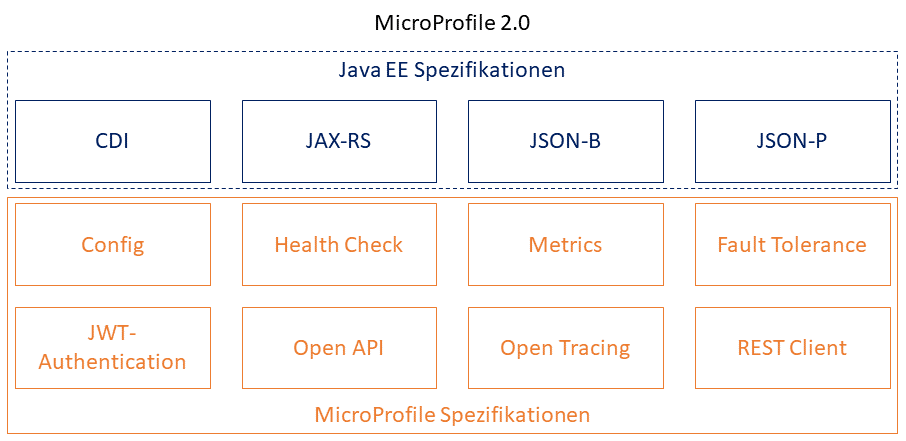
\includegraphics[width=\textwidth, center]{anhanga/microprofile_components}
	\caption[Beschreibung für Verzeichnis2]{Bildunterschrift2}
	\label{img:microprofile_components}
\end{figure}

\end{document}
